\chapter{DishBrain}
\chaptermark{DishBrain}
\label{sec:dishbrain}
\begin{chaptergoals}
\item comment DishBrain code la balle par lieu et fréquence, et lit la raquette en différence de comptes;
\item pourquoi un comptage sur $10\ms$ est bruité, si bien que le réseau ne peut déplacer que la moyenne;
\item comment secouer le réseau après les seuls ratés le fait dériver vers les réglages qui ratent moins;
\item ce qui a été mesuré, ce qui est débattu, et comment reconstruire le banc pour tester le mécanisme.
\end{chaptergoals}

\section{Un réseau en boîte de culture joue au tennis}

DishBrain, c'est le nom que les auteurs ont donné au banc sur lequel une culture de neurones vivants, cultivée sur une puce à électrodes, joue à un tennis simplifié à une seule raquette~\cite{Kagan2022}. C'est l'expérience la plus débattue sur une machine faite de neurones vivants (ces machines sont passées en revue au chapitre~\ref{sec:livingmachine}), et elle est particulièrement commode pour notre livre. Ici, le petit réseau est accessible en entier: chaque entrée est fixée par l'expérimentateur, chaque sortie est enregistrée. Toutes les questions des chapitres précédents (comment le signal est codé, qui enseigne, ce que voit la sonde) peuvent être posées à un réseau qui n'a ni yeux, ni muscles, ni neurones \nt{DOPA}. Analysons l'expérience comme un ingénieur analyse le banc d'un autre: schéma, entrée, sortie, professeur, résultat, controverses.

\section{Le banc}

Les neurones proviennent du cortex d'embryons de souris, environ $800\,000$ cellules par puce, ou sont obtenus à partir de cellules souches humaines, environ un million par puce. Pendant quelques semaines, ils poussent sur la puce, s'interconnectent et commencent à émettre spontanément des impulsions et des bouffées. Sous eux, sur une surface de $8$~mm$^2$, se trouvent $26\,000$ électrodes de platine; on peut en enregistrer jusqu'à $1024$ simultanément, et en pratique on stimule par huit d'entre elles.

Une boucle est refermée autour de la culture (fig.~\ref{fig:dishloop}). Un ordinateur simule le jeu: la balle vole, rebondit sur les murs, la raquette monte et descend. La position de la balle est convertie en courant sur huit électrodes \og sensorielles\fg{}. Les impulsions de deux zones \og motrices\fg{} sont comptées par fenêtres de $10\ms$ et déplacent la raquette. Après chaque renvoi ou raté, la culture reçoit un stimulus supplémentaire: la rétroaction. Les fenêtres de $10\ms$ sont le cycle de l'ordinateur du banc, et non celui de la culture: le réseau lui-même fonctionne toujours de façon asynchrone, comme tous les réseaux de ce livre.

\begin{figure}[t]
\centering
\begin{tikzpicture}[>=Stealth,
  blk/.style={draw,very thick,rounded corners=3pt,align=center,font=\small,minimum height=1.2cm},
  lab/.style={font=\scriptsize,align=center}]
\node[blk,fill=blue!6,text width=3.4cm] (C) at (0,0) {culture sur puce\\\scriptsize $\sim10^6$ neurones, $26\,000$ électrodes};
\node[blk,fill=orange!10,text width=3.0cm] (G) at (7.2,0) {ordinateur:\\partie de tennis};
\draw[->,very thick,blue!60!black] (G.north west) to[bend right=25] node[lab,above] {balle: \emph{lieu}, laquelle des 8 électrodes;\\\emph{fréquence}, 4--40 imp./s} (C.north east);
\draw[->,very thick,red!70!black] (C.south east) to[bend right=25] node[lab,below] {raquette: impulsions des zones\\\og haut\fg{} et \og bas\fg{} comptées sur $10\ms$} (G.south west);
\draw[->,thick,densely dashed,green!45!black] (G.east) -- ++(0.9,0) |- ++(0,-2.6) -| node[lab,pos=0.25,below] {renvoi: stimulus prévisible; raté: imprévisible} (C.south);
\end{tikzpicture}
\caption{La boucle DishBrain. Flèche bleue: l'entrée; la position de la balle est codée par un code de place et un code de fréquence (chapitre~\ref{sec:code}). Flèche rouge: la sortie; la différence des comptes des deux zones déplace la raquette. Flèche verte en tirets: la rétroaction après chaque échange, seul \og professeur\fg{} du banc.}
\label{fig:dishloop}
\end{figure}

\section{Entrée et sortie}

L'\emph{entrée} est codée à la fois par deux codes du chapitre~\ref{sec:code}. L'électrode stimulée, parmi les huit, indique à quelle hauteur se trouve la balle: c'est un code de place, comme celui des capteurs du chapitre~\ref{sec:sensors}. La cadence des impulsions de stimulation indique à quelle distance est la balle: $4$ par seconde quand elle est près du mur du fond, et davantage, linéairement, jusqu'à $40$ par seconde quand elle est près du mur de la raquette. C'est un code de fréquence; l'amplitude des impulsions de la balle est de $75$~mV. La culture ne \og connaît\fg{} d'avance aucun de ces codes: le code est fixé par l'expérimentateur, et le réseau doit apprendre à le lire.

La \emph{sortie} se lit comme dans les interfaces du chapitre~\ref{sec:debugging}. Les impulsions d'une zone motrice poussent la raquette vers le haut, celles de l'autre vers le bas; dans l'écriture la plus simple, pour chaque fenêtre,
\begin{empheq}[box=\keybox]{equation}
\Delta p \;=\; c\,\bigl(n_\uparrow - n_\downarrow\bigr),
\label{eq:dishreadout}
\end{empheq}
où $n_\uparrow$, $n_\downarrow$ sont les nombres d'impulsions des deux zones en $10\ms$, et $c$ un coefficient du banc. C'est le code à deux fils du chapitre~\ref{sec:glutcomputer}: le sens du mouvement n'est pas porté par le signe du signal, mais par celui des deux fils qui parle le plus fort.

Examinons le bruit d'une telle sortie. Si une zone émet au total $R$ impulsions par seconde, une fenêtre $T=10\ms$ en contient en moyenne $RT$, et d'après~\eqref{eq:rateerror} la dispersion relative vaut $1/\sqrt{RT}$. Pour $R=1000$ impulsions par seconde, cela fait environ $30$ pour cent dans chaque fenêtre; pour $R=100$, plus de cent. La raquette tremble inévitablement, et le réseau ne peut apprendre que d'une seule façon: en décalant la différence \emph{moyenne} des comptes dans le bon sens. Ce sont les mêmes lois qui limitent toute interface du chapitre~\ref{sec:debugging}, mais cette fois des deux côtés de la boucle.

\section{Un professeur sans dopamine}

Le plus intéressant, sur ce banc, c'est le professeur. Une culture de neurones du cortex ne contient pas de neurones \nt{DOPA}, et le banc n'envoie aucun signal \og mieux que prévu\fg{}. La rétroaction est d'une autre nature. Si le réseau renvoie la balle, un bref stimulus \emph{prévisible} est appliqué simultanément aux huit électrodes sensorielles: des impulsions de $75$~mV, $100$ par seconde pendant $0.1\,\text{s}$. S'il la rate, un stimulus que les auteurs qualifient d'\emph{imprévisible} dure quatre secondes: des impulsions de $150$~mV, $5$ par seconde, à des instants aléatoires et sur des électrodes tirées au hasard; suivent quatre secondes de pause sans stimulation, puis la balle repart~\cite{Kagan2022}.

Les auteurs partaient de l'hypothèse que le réseau agit de façon à rendre son entrée prévisible~\cite{Friston2010}. Pour un ingénieur, le sens est simple: la culture n'a qu'un moyen d'échapper à quatre secondes de bruit aléatoire, renvoyer la balle. Nous avons déjà rencontré la même idée dans l'économie d'impulsions du chapitre~\ref{sec:code} et dans la prédiction d'image du chapitre~\ref{sec:recognition}.

Mais la prévisibilité est-elle vraiment nécessaire ici? Un mécanisme plus grossier est possible. Supposons que le stimulus imprévisible après un raté se contente de \emph{brasser} les changements récents du réseau, tandis que le stimulus calme après un renvoi n'y touche pas. Décrivons le réglage du réseau par un vecteur $\boldsymbol\psi$, et soit $P_{\text{raté}}(\boldsymbol\psi)$ la probabilité de rater avec le réglage $\boldsymbol\psi$. Si les secousses sont symétriques (passer de $\boldsymbol\psi$ à $\boldsymbol\psi'$ est aussi probable que l'inverse), alors en régime établi le flux de départs de chaque réglage est équilibré par le flux d'arrivées, et la fraction du temps que le réseau passe dans le réglage $\boldsymbol\psi$ vaut
\begin{empheq}[box=\keybox]{equation}
\rho(\boldsymbol\psi) \;\propto\; \frac{1}{P_{\text{raté}}(\boldsymbol\psi)} .
\label{eq:dishdensity}
\end{empheq}
Un réglage qui rate dix fois moins souvent est conservé dix fois plus longtemps. Personne n'indique au réseau dans quel sens modifier ses poids: les bons réglages sont simplement détruits moins souvent.

Nous l'avons vérifié sur un modèle qui réduit la culture à deux nombres: la raquette arrive au point $a\,y+b$ quand la balle arrive à la hauteur $y$, et elle renvoie si l'écart est inférieur à $0.1$. Après un raté, les deux nombres reçoivent une secousse aléatoire; après un renvoi, ils restent inchangés. Sur $2000$ échanges, la proportion de balles renvoyées est passée de $0.21$ sur les deux cents premiers à $0.38$ sur les cinq cents derniers (quarante \og cultures\fg{}, fig.~\ref{fig:dishmodel}). Si l'on applique la secousse après \emph{chaque} échange, la rétroaction ne porte aucune information, et la proportion reste vers $0.12$; sans aucune secousse, elle reste à $0.19$. L'expérience sur le banc concorde: une hausse significative au cours d'une session n'apparaissait qu'avec la rétroaction complète. Avec du silence à la place des stimuli, la culture jouait tout de même mieux en fin de session que sans rétroaction, mais avec un effet moindre~\cite{Kagan2022}; notons que, dans cette condition aussi, un raté est suivi d'une longue pause et un renvoi d'une pause courte, de sorte que la différence entre les issues ne disparaît pas entièrement.

\begin{figure}[t]
\centering
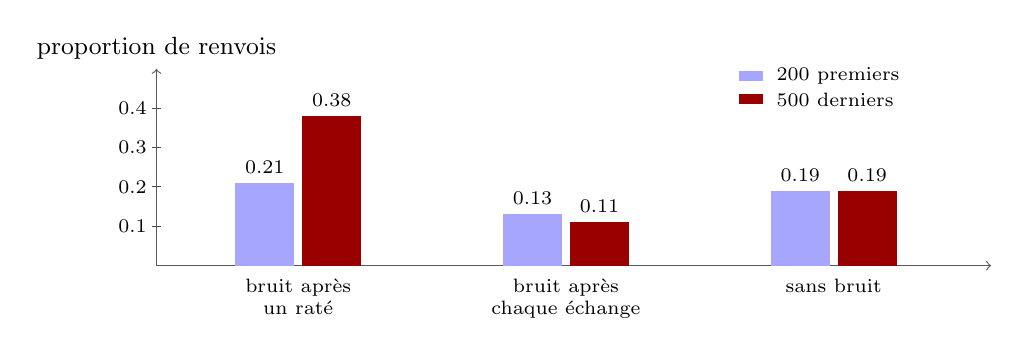
\begin{tikzpicture}[x=1cm,y=5cm]
\draw[->,gray!70!black] (0,0) -- (10.6,0);
\draw[->,gray!70!black] (0,0) -- (0,0.5) node[above,font=\small,black] {proportion de renvois};
\foreach \v in {0.1,0.2,0.3,0.4}{\draw[gray!60!black] (-0.06,\v) -- (0.06,\v); \node[left,font=\scriptsize] at (0,\v) {\v};}
\foreach \x/\f/\l/\lab in {1.8/0.21/0.38/{bruit après\\un raté},5.2/0.13/0.11/{bruit après\\chaque échange},8.6/0.19/0.19/{sans bruit}}{
  \fill[blue!35] (\x-0.8,0) rectangle (\x-0.05,\f);
  \fill[red!60!black] (\x+0.05,0) rectangle (\x+0.8,\l);
  \node[below,font=\scriptsize,align=center] at (\x,-0.01) {\lab};
  \node[above,font=\scriptsize] at (\x-0.425,\f) {\f};
  \node[above,font=\scriptsize] at (\x+0.425,\l) {\l};}
\fill[blue!35] (7.4,0.47) rectangle (7.7,0.495); \node[right,font=\scriptsize] at (7.75,0.482) {200 premiers};
\fill[red!60!black] (7.4,0.41) rectangle (7.7,0.435); \node[right,font=\scriptsize] at (7.75,0.422) {500 derniers};
\end{tikzpicture}
\caption{Modèle du \og brassage après un raté\fg{} (\texttt{dishbrain\_model.py}): proportion de balles renvoyées au début et à la fin de $2000$ échanges, moyenne sur quarante cultures modèles. L'apprentissage n'a lieu que si la secousse suit un raté et non un renvoi, comme dans l'expérience, où la hausse significative en une session n'apparaissait qu'avec la rétroaction complète.}
\label{fig:dishmodel}
\end{figure}

\begin{keyblock}
\begin{proposition}[Le professeur brasseur]
\label{prop:dishscramble}
Si l'échec secoue le réseau et que le succès le laisse en paix, le réseau dérive de lui-même vers les réglages qui se trompent moins souvent: le temps passé dans un réglage est inversement proportionnel à la probabilité d'échec~\eqref{eq:dishdensity}. Un tel apprentissage n'exige ni signal de récompense, ni signe de ce signal, ni prévisibilité en tant que telle: il suffit que la rétroaction après un succès diffère de celle qui suit un échec. Le changement de comportement de la culture est mesuré; le mécanisme à l'œuvre dans la boîte (prédiction de l'entrée ou brassage) n'est pas établi.
\end{proposition}
\end{keyblock}

Comparez avec le chapitre~\ref{sec:dofa}. Là aussi, le bruit servait à la recherche, mais la dopamine avait un signe: l'erreur $\delta$ indiquait dans quel sens déplacer les poids, et le pas suivait le gradient~\eqref{eq:perturbation}. Ici, il n'y a pas de signe, seulement \og garder\fg{} ou \og secouer\fg{}. Une telle recherche est plus grossière et plus lente, mais elle exige moins du réseau: ni neurones \nt{DOPA}, ni critique, ni trace étalée sur des secondes.

\section{Ce qui a été mesuré et ce qui est débattu}

Chaque partie durait $20$ minutes; on comparait les $5$ premières minutes aux $15$ dernières. Chez les cultures à rétroaction complète, les séries de renvois se sont allongées et les ratés immédiats sont devenus plus rares; dans les contrôles sans cellules, sans jeu ou avec une \og raquette\fg{} pilotée par ordinateur, rien de tel. Les cultures de cellules humaines tenaient en moyenne plus longtemps que celles de souris. L'amélioration est statistiquement robuste (sur neuf cultures de souris et onze cultures humaines, dans une bonne centaine de parties par groupe), mais modeste: le réseau n'est pas devenu un bon joueur, il est devenu un peu meilleur que le hasard. Elle est robuste au sein d'une session; les auteurs n'ont pas obtenu d'apprentissage stable d'une session à l'autre sur plusieurs jours~\cite{Kagan2022}. Un travail ultérieur du même groupe a montré que, pendant le jeu, l'activité de la culture se rapproche du régime \emph{critique}, la frontière entre extinction et avalanche, cette même vie au bord du gouffre qu'au chapitre~\ref{sec:gaba}, et que plus elle s'en approche, meilleur est le jeu~\cite{Habibollahi2023}.

La principale controverse n'a pas porté sur les chiffres, mais sur les mots. Le titre de l'article affirmait que les neurones en boîte \og font preuve de sensibilité\fg{} (sentience), et un groupe de chercheurs a objecté qu'un changement de comportement en boucle fermée n'est encore ni intelligence ni sensation, et que les conclusions doivent être formulées plus modestement~\cite{Balci2023}. Du point de vue de l'ingénieur, deux questions restent ouvertes, et toutes deux portent sur le mécanisme. Première question: le réseau apprend-il, c'est-à-dire ses poids changent-ils durablement, ou la rétroaction ne fait-elle que décaler son état courant? Seconde question: la prévisibilité est-elle réellement nécessaire, ou toute différence entre la réponse au succès et la réponse à l'échec suffit-elle, comme dans la proposition~\ref{prop:dishscramble}? Un banc où chaque électrode est accessible permet de répondre aux deux, et c'est sans doute là sa principale valeur.

\section{Spécification du banc: comment le reproduire}
\label{sec:dishspec}

On trouvera ci-dessous tout ce qu'il faut pour reconstruire un tel banc: matériel, boucle, codage de l'entrée, lecture de la sortie, rétroaction et protocole expérimental. Chaque paramètre est marqué de sa source. \og Article\fg{}: la valeur est tirée du texte de l'étude~\cite{Kagan2022}. \og Choix\fg{}: l'article ne la donne pas, et il faudra la fixer soi-même pour reproduire l'expérience; nous proposons une valeur par défaut et indiquons comment la vérifier.

\subsection*{Matériel et culture}

\begin{center}
\footnotesize
\setlength{\tabcolsep}{4pt}
\renewcommand{\arraystretch}{1.15}
\begin{tabular}{>{\raggedright}p{4.0cm}>{\raggedright}p{6.9cm}>{\raggedright\arraybackslash}p{1.6cm}}
\toprule
Paramètre & Valeur & Source \\
\midrule
puce & matrice MaxOne: $26\,000$ électrodes de platine sur une surface de $8$~mm$^2$ & article \\
enregistrement & jusqu'à $1024$ canaux simultanés, $20\,000$ échantillons par seconde & article \\
stimulation & jusqu'à $32$ électrodes techniquement, $8$ indépendantes dans l'expérience & article \\
cellules & cortex d'embryon de souris; neurones humains issus de cellules souches (deux méthodes de culture); cellules HEK293T (non neuronales) comme contrôle & article \\
ensemencement & environ $10^6$ cellules par puce & article \\
âge de la culture lors de l'expérience & souris: à partir de $\sim10$ jours; humain: $14$--$24$ jours ou $\sim80$ jours selon la méthode de culture & article \\
\bottomrule
\end{tabular}
\end{center}

\subsection*{Boucle et temps}

La boucle fonctionne par fenêtres de $10\ms$ ($200$ échantillons): pendant chaque fenêtre, on compte les impulsions sur les électrodes des zones motrices, le jeu est mis à jour et la stimulation suivante est émise. Le délai entre une impulsion dans la culture et le stimulus de réponse est d'environ $5\ms$. Pendant le jeu, le signal de chaque électrode passe par un filtre passe-haut de Bessel d'ordre 2 de fréquence de coupure $100$~Hz; la valeur absolue du signal est lissée par un filtre passe-bas de Bessel d'ordre 1 à $1$~Hz, et le seuil de détection des impulsions est proportionnel à cette valeur absolue lissée. Le seuil de six écarts types du fond, l'article l'indique pour certaines mesures d'activité, et non pour le jeu. Pour que la stimulation ne soit pas comptée comme une réponse de la culture, tous les signaux sont masqués lorsque plus de $15$ grandes impulsions, au-dessus de $75$~mV, arrivent en même temps. Tout ceci: article.

\subsection*{Codage de la balle}

\begin{center}
\footnotesize
\setlength{\tabcolsep}{4pt}
\renewcommand{\arraystretch}{1.15}
\begin{tabular}{>{\raggedright}p{3.4cm}>{\raggedright}p{7.5cm}>{\raggedright\arraybackslash}p{1.6cm}}
\toprule
Paramètre & Valeur & Source \\
\midrule
zone sensorielle & $8$ électrodes disposées de sorte que des électrodes voisines correspondent à des positions voisines de la balle & article \\
code de place & le numéro d'électrode $k=1,\dots,8$ indique la position de la balle par rapport au centre de la raquette & article \\
quelle coordonnée & position verticale de la balle; pour la reproduction, par rapport à la raquette, $k=\lceil 8(y-p+\tfrac12)\rceil$ pour $y-p\in[-\tfrac12,\tfrac12]$ & article; formule: choix \\
code de fréquence & la fréquence de stimulation, de $4$ à $40$~imp./s, porte la distance à la raquette & article \\
sens de l'échelle & $4$~imp./s quand la balle est près du mur opposé, et linéairement jusqu'à $40$~imp./s près du mur de la raquette: $f=4+36\,(1-x/L)$, $x$ étant la distance au mur de la raquette et $L$ la largeur du court & article \\
forme d'impulsion & brève impulsion rectangulaire biphasique: d'abord la phase positive, puis la négative & article \\
amplitude & $75$~mV; choisie pour ne pas forcer la décharge des cellules inhibées & article \\
durée des phases & non indiquée; prendre le réglage standard du système de stimulation et ne pas le modifier pendant l'expérience & choix \\
\bottomrule
\end{tabular}
\end{center}

\subsection*{Lecture de la raquette}

L'article comporte deux zones motrices: les impulsions de la première déplacent la raquette vers le haut, celles de la seconde vers le bas; la contribution des zones est pondérée pour tenir compte de densités de cellules et d'activités différentes~\cite{Kagan2022}. La formule exacte n'est pas donnée. Pour la reproduction, nous prenons la règle~\eqref{eq:dishreadout}, $\Delta p=c\,(n_\uparrow-n_\downarrow)$ pour chaque fenêtre de $10\ms$, avec un poids qui égalise les zones selon leur activité moyenne au repos (choix): $n_\uparrow$ et $n_\downarrow$ sont divisés par le compte moyen de leur zone par fenêtre, mesuré avant le jeu. Le coefficient $c$ est choisi de sorte qu'une différence d'un compte moyen déplace la raquette de $1\%$ de la hauteur du court par fenêtre (choix); un avantage constant d'une zone fait alors traverser tout le court à la raquette en $1$~s.

L'emplacement des zones sur la puce n'est pas donné par des coordonnées dans le texte de l'article; il n'y a qu'un schéma. Pour la reproduction, trois groupes d'électrodes disjoints suffisent: les huit électrodes sensorielles au centre et, de part et d'autre, un groupe d'électrodes d'enregistrement, l'un pour \og haut\fg{}, l'autre pour \og bas\fg{} (choix).

\subsection*{Le jeu}

Les dimensions du court, la longueur de la raquette et la vitesse de la balle ne sont pas indiquées dans l'article; il est seulement dit que la balle se déplace à vitesse constante et rebondit sur les murs. Pour la reproduction (choix): court de $1\times1$, raquette de longueur $0.2$ sur le mur de droite (renvoi si $|y-p|<0.1$, comme dans le modèle~\texttt{models/dishbrain\_model.py}), la balle traverse le court en $1$~s. Un raté sans aucun renvoi dans l'échange compte comme un \og ace\fg{}; un échange de plus de trois renvois consécutifs est dit \og long\fg{} (article).

\subsection*{Rétroaction}

\begin{center}
\footnotesize
\setlength{\tabcolsep}{4pt}
\renewcommand{\arraystretch}{1.15}
\begin{tabular}{>{\raggedright}p{2.6cm}>{\raggedright}p{8.3cm}>{\raggedright\arraybackslash}p{1.6cm}}
\toprule
Événement & Ce qui est appliqué & Source \\
\midrule
renvoi & stimulus prévisible: les $8$ électrodes sensorielles simultanément, $75$~mV, $100$~imp./s, $100\ms$; la stimulation habituelle de la balle est interrompue pendant ce temps & article \\
raté & stimulus imprévisible: $150$~mV, $5$~imp./s, $4$~s, à des instants aléatoires sur des électrodes tirées au hasard parmi les $8$; puis $4$~s sans stimulation, et la balle repart dans une direction aléatoire & article \\
loi du hasard & non indiquée; pour la reproduction, instants des impulsions en flux de Poisson de fréquence moyenne $5$~imp./s & choix \\
\bottomrule
\end{tabular}
\end{center}

\subsection*{Protocole et contrôles}

Une session dure $20$~min; on compare les $5$ premières et les $15$ dernières minutes (article). Trois mesures du résultat: la longueur moyenne d'un échange, la proportion d'aces et la proportion d'échanges longs. Conditions expérimentales (article):
\begin{itemize}
\item \emph{stimulus}: boucle complète, telle que décrite ci-dessus;
\item \emph{silence}: au lieu du stimulus de renvoi ou de raté, la même durée sans aucune stimulation, puis la balle repart dans une direction aléatoire;
\item \emph{sans rétroaction}: après un raté, la balle rebondit simplement et continue sa course, et la stimulation de la position de la balle se poursuit;
\item \emph{repos}: le jeu tourne et la raquette suit l'activité, mais il n'y a aucune stimulation;
\item \emph{contrôles}: puce avec milieu seul; cellules HEK293T; \og culture in silico\fg{}, une simulation à la place des cellules.
\end{itemize}
Taille des échantillons dans la série principale: $9$ cultures de souris ($101$ sessions), $11$ cultures humaines ($138$), $6$ puces avec milieu seul ($80$), $20$ cultures au repos ($42$), $3$ simulations ($38$), soit $399$ sessions au total. Dans la série sur la rétroaction: $486$ sessions sur $3$ jours, à raison de $3$ sessions par jour, conditions \og stimulus\fg{}, \og silence\fg{} et \og sans rétroaction\fg{} ($n=27$, $17$ et $15$). La hausse de la longueur moyenne des échanges entre les $5$ premières minutes et les $15$ dernières n'a été obtenue qu'avec des cultures vivantes. Dans la série sur la rétroaction, une hausse significative au fil du temps n'apparaît que dans la condition \og stimulus\fg{}; en fin de session, la condition \og silence\fg{} dépassait tout de même \og sans rétroaction\fg{}, mais avec un effet moindre, et il n'y a pas eu d'apprentissage stable d'une session à l'autre sur les trois jours~\cite{Kagan2022}.

\subsection*{Le cycle du banc pas à pas}

Toutes les $10\ms$, l'ordinateur du banc effectue les opérations suivantes.
\begin{enumerate}
\item Il lit les nombres d'impulsions $n_\uparrow$, $n_\downarrow$ des deux zones motrices sur la fenêtre écoulée et les normalise par le compte moyen de la zone au repos.
\item Il déplace la raquette de $\Delta p=c\,(n_\uparrow-n_\downarrow)$ et la maintient dans les limites du court.
\item Il avance la balle d'un pas et la fait rebondir sur les murs du haut, du bas et de gauche.
\item Si la balle a atteint le mur de droite: pour $|y-p|<0.1$, c'est un renvoi, le compteur de l'échange augmente d'une unité et le stimulus de renvoi est appliqué ($100\ms$); sinon, c'est un raté, l'échange est enregistré, le stimulus de raté est appliqué ($4$~s), suivi de $4$~s de pause, et la balle repart.
\item Sinon, il choisit l'électrode $k$ d'après la position verticale de la balle et la fréquence $f$ d'après la distance au mur de la raquette, et applique à l'électrode $k$ des impulsions biphasiques de $75$~mV à la fréquence $f$ jusqu'à la fenêtre suivante.
\end{enumerate}
Cela suffit pour construire un banc compatible avec celui qui a été publié et pour tester la question centrale du chapitre: est-ce la prévisibilité qui enseigne à la culture, ou la simple différence entre la réponse au renvoi et celle au raté? Pour cela, il faut ajouter aux trois conditions de l'article une quatrième, qui n'y figure pas: après un raté, un stimulus \emph{prévisible} de même durée et de même énergie que le stimulus imprévisible. Si la culture apprend aussi dans ce cas, c'est la différence qui compte, et non la prévisibilité.


\section{Bilan}

\begin{table}[t]
\centering
\footnotesize
\setlength{\tabcolsep}{4pt}
\renewcommand{\arraystretch}{1.15}
\begin{tabular}{>{\raggedright}p{2.1cm}>{\raggedright}p{4.2cm}>{\raggedright}p{1.9cm}>{\raggedright\arraybackslash}p{4.6cm}}
\toprule
Bloc du banc & Fonctionnement & Chapitre du livre & Ce que l'on sait \\
\midrule
entrée & lieu (laquelle des 8 électrodes) et fréquence (4--40 imp./s) & \ref{sec:code}, \ref{sec:sensors} & fixée par l'expérimentateur \\
sortie & différence des comptes des deux zones en $10\ms$~\eqref{eq:dishreadout} & \ref{sec:glutcomputer}, \ref{sec:debugging} & fixée par l'expérimentateur; bruit selon~\eqref{eq:rateerror} \\
professeur & stimulus prévisible après un renvoi, imprévisible après un raté; pas de dopamine & \ref{sec:dofa} & hausse significative en une session seulement avec rétroaction complète; effet moindre avec le silence; instable d'une session à l'autre \\
mécanisme & prédiction de l'entrée ou brassage après un raté~\eqref{eq:dishdensity} & \ref{sec:dofa}, \ref{sec:recognition} & non établi; les deux expliquent le résultat \\
régime du réseau & rapprochement du régime critique pendant le jeu & \ref{sec:gaba} & lien avec la qualité du jeu mesuré \\
\og sensibilité\fg{} & affirmation des auteurs & --- & non démontrée; contestée \\
\bottomrule
\end{tabular}
\caption{DishBrain vu par un ingénieur.}
\label{tab:dishbrain}
\end{table}

DishBrain est une machine faite de neurones vivants sous sa forme la plus simple: l'entrée est fixée par un code, la sortie lue par un comptage, et le professeur est la différence entre la réponse au succès et la réponse à l'échec (tableau~\ref{tab:dishbrain}). Un réseau sans yeux, sans muscles et sans dopamine a appris à jouer un tout petit peu, et cela seul en fait un banc d'essai pour les idées du livre. Quel que soit le mécanisme (prédiction, brassage ou autre chose), la réponse sera trouvée comme le conseille le chapitre~\ref{sec:debugging}: avec une sonde, un signal de test et la mise hors circuit de certaines parties, sur une machine que l'on voit enfin en entier.

\section{Exercices}

\begin{exercise}[\lvlA]
\label{ex:22:1}
\emph{De combien décaler le compte.} Les deux zones émettent ensemble $R_\uparrow+R_\downarrow=2000$ impulsions par seconde, flux poissoniens. (a)~Dispersion relative du compte d'une zone en $10\ms$ pour $R=1000$ et $R=100$? (b)~En $1$~s de vol de la balle, les déplacements~\eqref{eq:dishreadout} s'additionnent. Plus petit $R_\uparrow-R_\downarrow$ donnant un déplacement moyen double de la dispersion?
\end{exercise}

\begin{exercise}[\lvlA]
\label{ex:22:2}
\emph{Combien d'échanges pour voir l'apprentissage.} Les échanges sont indépendants, la proportion de renvois est binomiale. Combien d'échanges faut-il dans chacune des deux périodes pour que la hausse de la proportion de renvois dépasse deux écarts types de la différence: (a)~de $0.20$ à $0.25$; (b)~de $0.21$ à $0.38$, comme dans le modèle?
\end{exercise}

\begin{exercise}[\lvlB]
\label{ex:22:3}
\emph{Démonstration de~\eqref{eq:dishdensity}.} Le réglage $\boldsymbol\psi$ parcourt un ensemble fini; en cas de raté (probabilité $P(\boldsymbol\psi)>0$), le réseau passe en $\boldsymbol\psi'$ avec une probabilité symétrique $K(\boldsymbol\psi,\boldsymbol\psi')$; en cas de renvoi, il reste. (a)~Démontrez que $\rho\propto1/P$ est la distribution stationnaire. (b)~Quelle est la proportion de ratés avec deux réglages où $P=0.9$ et $P=0.1$?
\end{exercise}

\begin{exercise}[\lvlB]
\label{ex:22:4}
\emph{La région absorbante du modèle.} La raquette arrive en $p=\min\bigl(1,\max(0,ay+b)\bigr)$, la balle à la hauteur $y\sim U(0,1)$, et il y a renvoi si $|p-y|<h=0.1$. (a)~Démontrez que pour $|b|<h$ et $|a-1+b|<h$ le réseau renvoie toutes les balles, et trouvez l'aire de cette région. (b)~Trouvez numériquement la proportion moyenne de renvois pour $a\sim U(-1,1)$, $b\sim U(0,1)$.
\end{exercise}

\begin{exercise}[\lvlB]
\label{ex:22:5}
\emph{Simulation: une clôture autour des réglages.} Dans une copie de \texttt{dishbrain\_model.py}, faites jouer $200$ cultures pendant $20\,000$ échanges chacune. Quelle est la proportion de renvois sur les $500$ derniers? Et si, après chaque secousse, on ramène le réglage dans le rectangle $a\in[-1,2]$, $b\in[-1,1]$? Expliquez la différence à l'aide de l'exercice~\ref{ex:22:3}.
\end{exercise}

\begin{exercise}[\lvlB]
\label{ex:22:6}
\emph{Conception du code d'entrée.} La balle est renvoyée si l'erreur de hauteur est inférieure à $h=0.1$; le réseau lit l'entrée en $T=0.25$~s et distingue environ $\sqrt{rT}$ niveaux jusqu'à la fréquence $r$; la stimulation ne dépasse pas $40$ impulsions par seconde. (a)~Un code de place sur huit électrodes suffit-il? (b)~Et la fréquence sur une seule électrode?
\end{exercise}

\begin{exercise}[\lvlC]
\label{ex:22:7}
\emph{Recherche: prédiction ou brassage?} Généralisez le modèle à $d$ nombres réglables ($p=\sum_{i<d}a_iy^i$). Comment le nombre d'échanges menant à $0.5$ de renvois croît-il avec $d$, par brassage et par la règle au signe de l'erreur~\eqref{eq:perturbation}? Quelle expérience sur le banc départagerait les deux hypothèses?
\end{exercise}
